\chapter{State of the Art and Technical Foundations}
\label{chap:background}

\section*{Introduction}

This chapter establishes the technical background on which the rest of the
report rests. The Energy Transition Optimizer is not only a Power-to-X model: it
is an analytical product that must be usable, maintainable, secure, and, with the
new conversational layer, assisted by language models without losing its
numerical authority. For this reason the state of the art is examined along
several axes rather than a single one.

The chapter is organized in four movements. It first studies the existing
platform as the concrete starting point of the project. It then lays the
technical foundations axis by axis, from techno-economic optimization to
language-model agents, and gives particular attention to two axes central to
this work: the interpretation and visualization of
results, and the evaluation of language-model behavior. It then benchmarks the
possible directions and justifies the one adopted. Finally, it positions the
work within that landscape.

\section{Analysis of the existing ETO platform}
\label{sec:existing}

The project did not start from a blank page. The existing Energy Transition
Optimizer already offered a working foundation for Power-to-X pre-feasibility
analysis: users could create projects, define assumptions, build a topology, run
simulations, and inspect numerical outputs. Studying it was essential, because it
made it possible to distinguish what had to be preserved from what had to be
redesigned.



\subsection{A valuable deterministic core}

The analytical core was, and remains, the most valuable part of the product. It
turns a declared topology and a set of assumptions into reproducible operating
schedules and financial indicators. This determinism is precisely what makes the
tool trustworthy for investment-oriented analysis: given the same inputs, it
returns the same result. Any evolution of the product therefore had to protect
this core rather than replace it.

\subsection{An expert-oriented workflow}

The workflow around the core, however, showed the limits of an internal,
expert-only tool. To obtain an answer, a user had to hand-build a valid topology,
bind library assumptions to each node, set sweep ranges across many parameters,
launch a grid search, and finally read a population of results. Each of these
steps assumed prior knowledge of the model and of the meaning of its parameters
(Figure~\ref{fig:experts}).
The tool was powerful for specialists but difficult to approach for the broader
set of analysts who could benefit from it.
\begin{figure}[H]
  \centering
  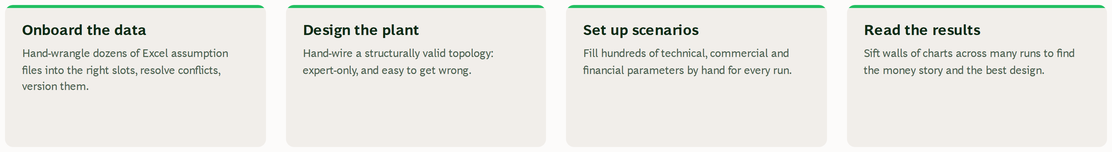
\includegraphics[width=\linewidth]{Figures/plant-workflow-bcg-style.png}
  \caption{An expert-only workflow: a bottleneck on every project.}
  \label{fig:experts}
\end{figure}

\subsection{Dated user experience and unsupported interpretation}

Two weaknesses were especially relevant to this work. First, the visual design
was dated and inconsistent across screens
(Figure~\ref{fig:existing-eto-platform}), which lowered the perceived maturity
of the product and eroded confidence during first use. Second, and more
importantly, \textbf{result interpretation was almost entirely unsupported}. The
platform could display a point on a chart or the status of a simulation, but it
did not explain whether a result was expected, which assumptions had driven it,
or what a user should do next. Turning a table of net present values and internal
rates of return into an operational and financial narrative was left entirely to
the user. This gap is the direct motivation for the interpretation and
visualization work presented later in this report.
\begin{figure}[H]
  \centering
  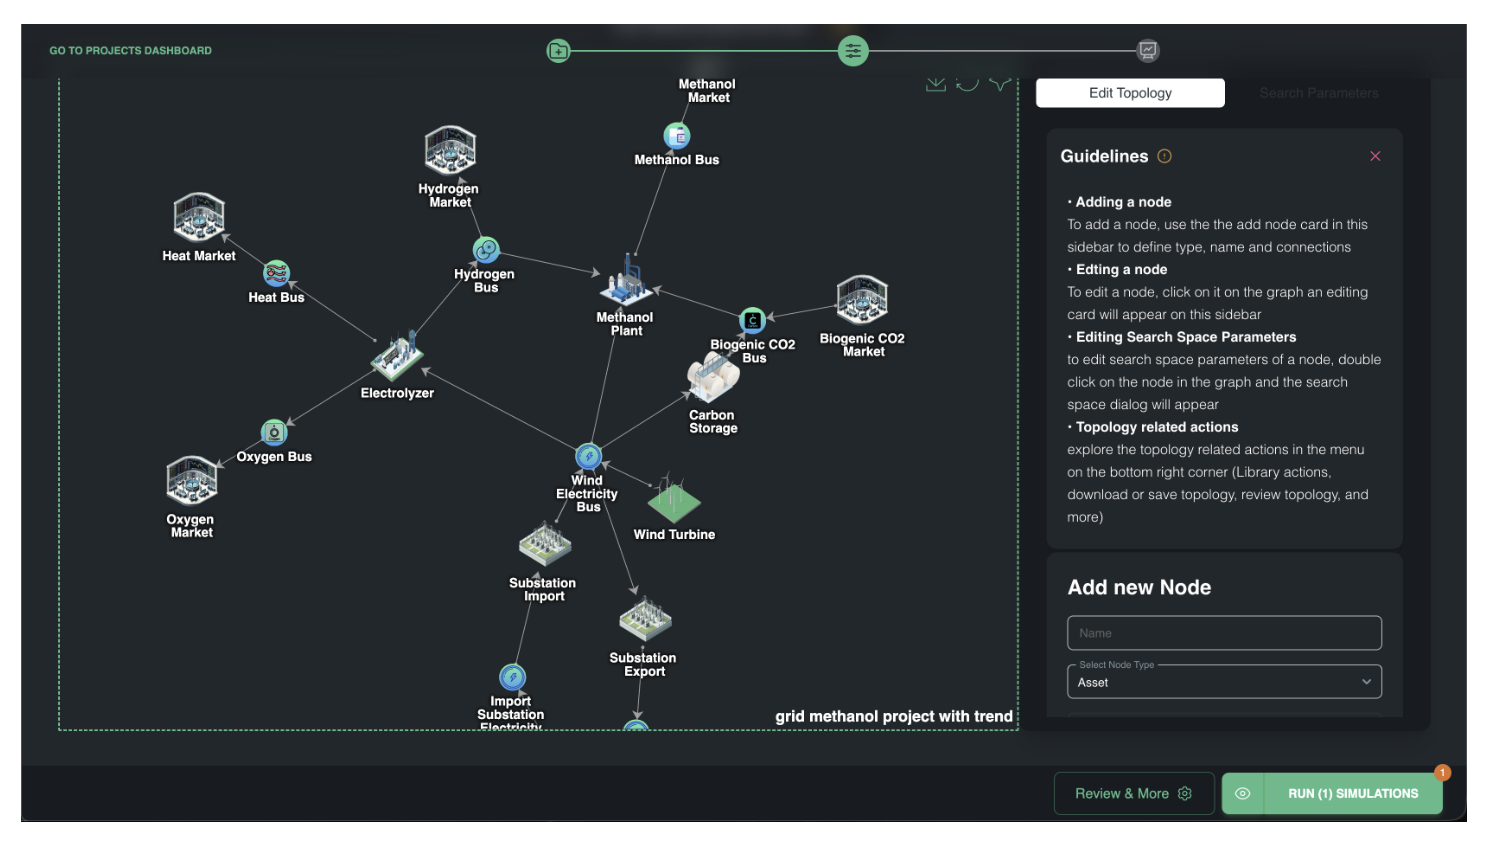
\includegraphics[width=0.48\linewidth]{Figures/old 1.png}
  \hfill
  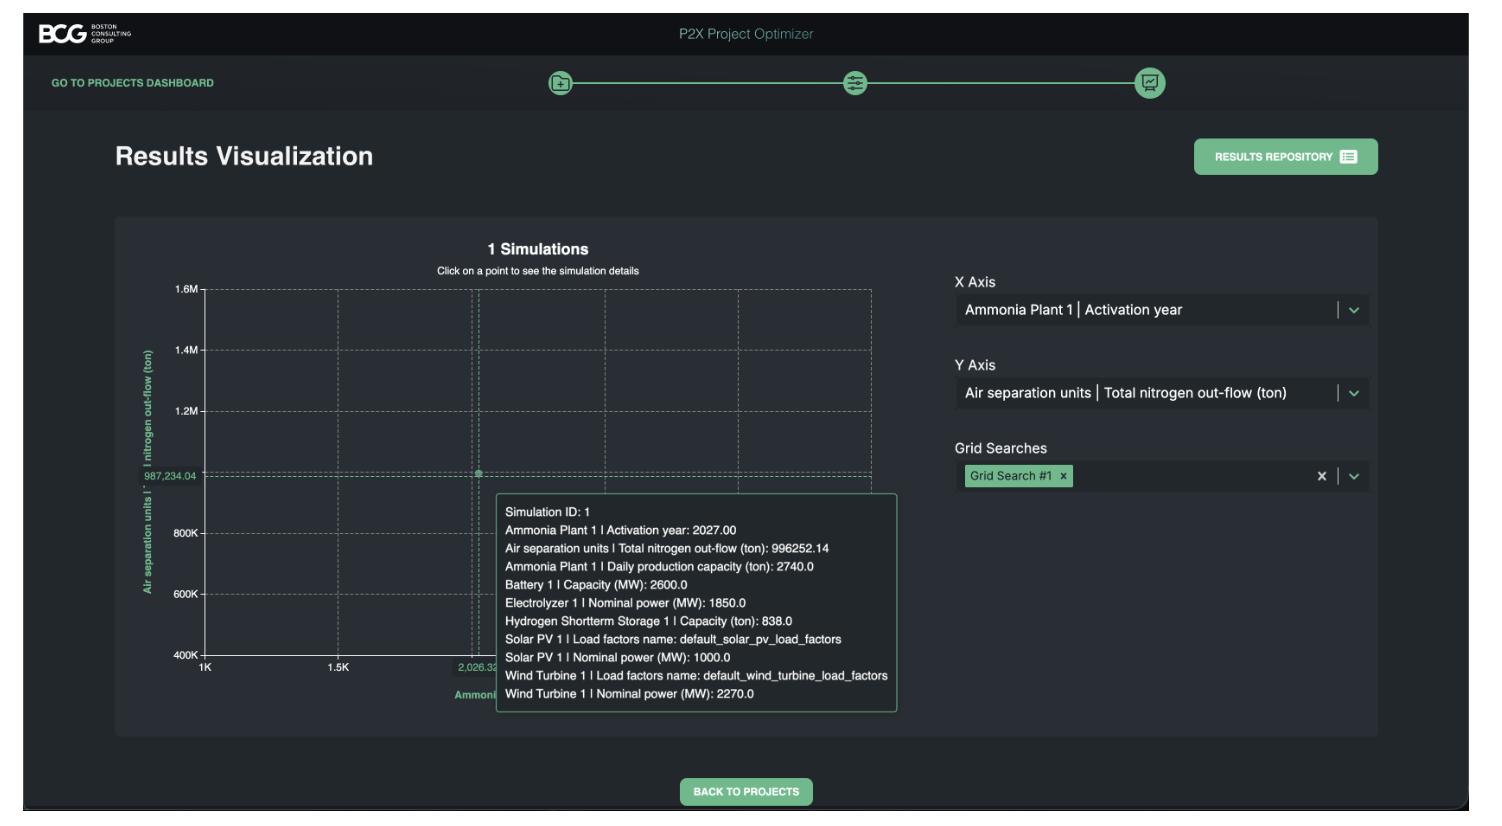
\includegraphics[width=0.48\linewidth]{Figures/old 2.png}
  \caption{Two screens of the existing Energy Transition Optimizer interface.}
  \label{fig:existing-eto-platform}
\end{figure}

\subsection{A fragile platform and inherited identity risk}

Beyond the analytical experience, the product sat on a fragile platform: an
unreliable release process, environments that had drifted from any documented
baseline, and limited operational observability. In parallel, the inherited
authentication layer relied on self-hosted identity components, which placed
identity-provider responsibilities (patching, configuration, monitoring) inside
the application stack and constituted a security and compliance risk in its own
right. These issues had to be addressed before the product could be safely
extended.

\subsection{Synthesis of limitations}

The study of the existing platform can be summarized as follows. The limitations
were not concentrated in one component; they appeared across the user journey:

\begin{itemize}
  \item the workflow was expert-oriented and required prior knowledge of the
    model;
  \item the visual design was dated and reduced confidence during first use;
  \item results were available but their interpretation was mostly unsupported;
  \item the platform lacked any assistance connecting user intent, model
    configuration, execution, and result analysis;
  \item authentication and deployment foundations required modernization before
    the product could scale safely.
\end{itemize}

The key observation is that the missing piece was not the solver, which was
sound, but the product surrounding it. This framing guides the rest of the
chapter and the direction ultimately chosen.

\section{Techno-economic optimization and Power-to-X modeling}
\label{sec:opt-foundations}

\subsection{Linear and mixed-integer programming}

The analytical core belongs to the family of solver-backed optimization tools.
\textbf{Linear programming} (LP) optimizes a linear objective subject to linear
constraints over continuous variables, and is solvable efficiently
\cite{bertsimas1997}. \textbf{Mixed-integer linear programming} (MILP) extends it
with integer or binary variables, which are required whenever discrete operating
states must be represented (for example a unit being on or off)
\cite{nemhauser1988}. Energy-system operation is naturally expressed in this
form: continuous variables carry flows, powers, and inventories, while binary
variables carry discrete commitment decisions, an approach that mirrors classical
unit-commitment modeling in power systems \cite{wood2013, morales2013}. MILP is
NP-hard in general, but modern branch-and-cut solvers make realistic instances
tractable.

\subsection{Multi-carrier energy systems and energy hubs}

A Power-to-X project couples several energy carriers and commodities:
electricity, hydrogen, heat, and downstream molecules such as ammonia or
methanol. Such systems are naturally described as \textbf{multi-carrier energy
systems}, or \emph{energy hubs}, in which conversion and storage units link
inputs and outputs across carriers \cite{geidl2007opf, geidl2007hub}. This is
exactly the abstraction used by the Energy Transition Optimizer, where a project
is a typed graph of assets, commodity-conservation buses, and markets. The
economic and climate relevance of these pathways for hard-to-abate sectors is
well documented \cite{ueckerdt2021, hermesmann2021}.

\begin{figure}[H]
  \centering
  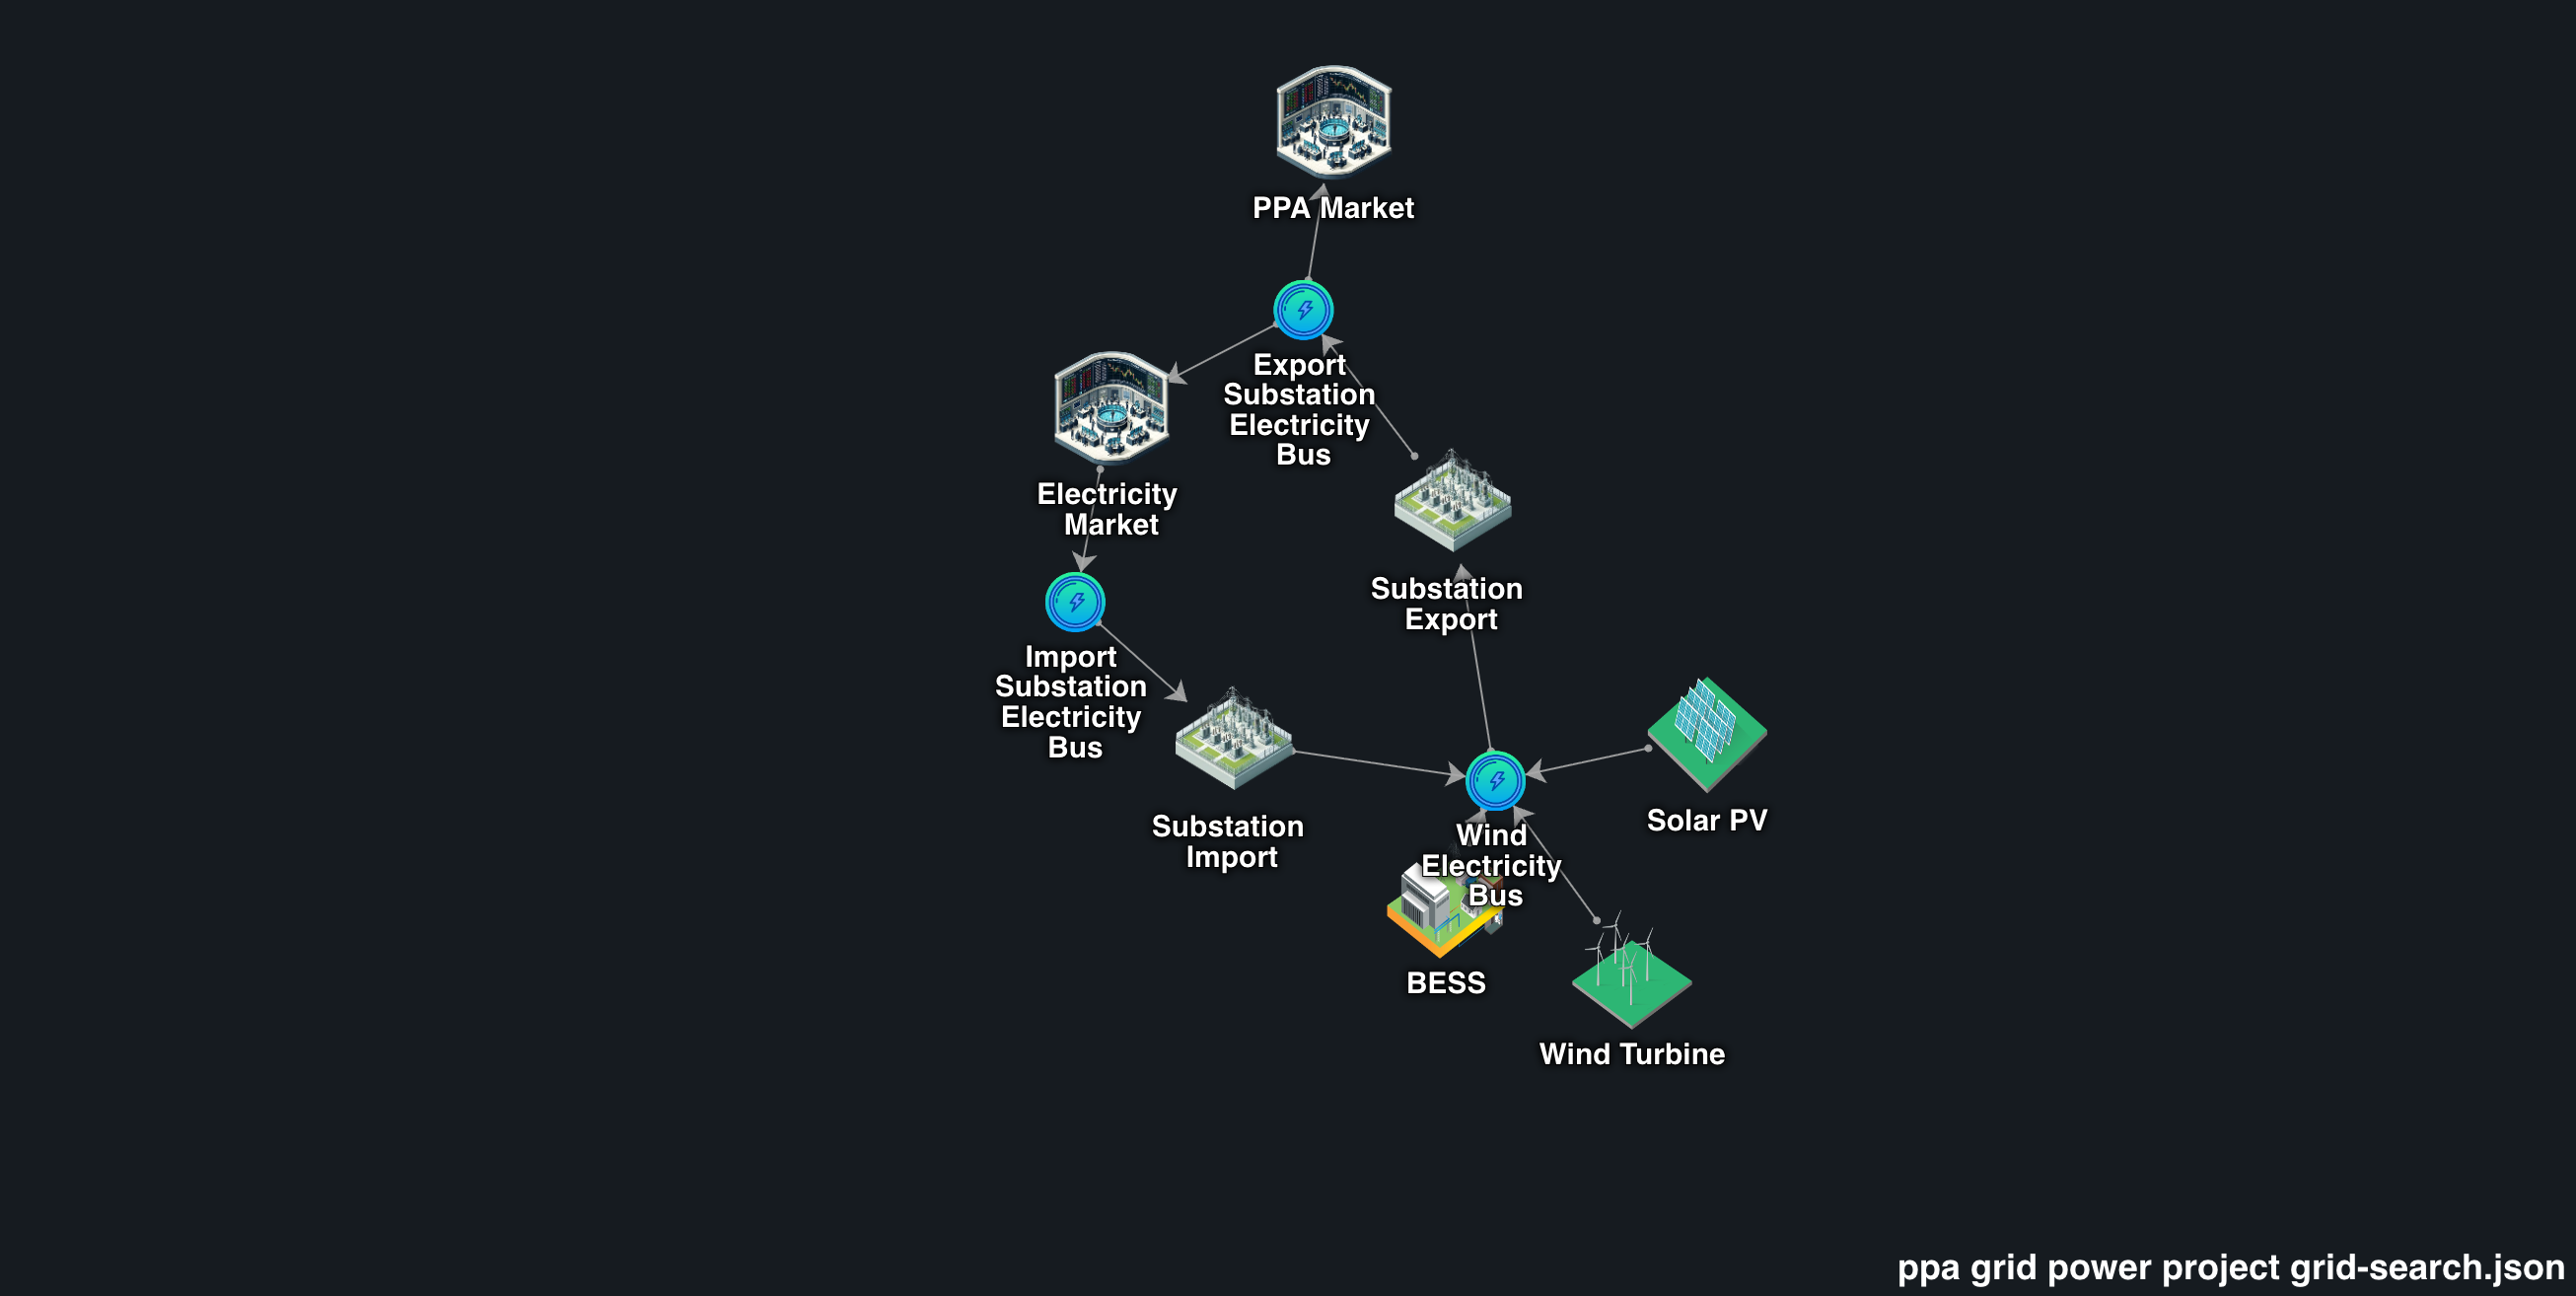
\includegraphics[width=0.8\linewidth]{Figures/energy_hub_example.png}
  \caption{An example multi-carrier topology (energy hub).}
  \label{fig:energy-hub-example}
\end{figure}

\newpage
Figure~\ref{fig:energy-hub-example} shows an example of such a topology.
Concretely, the operational problem solved over each planning window has the
general form of a (mixed-integer) linear program:
\begin{align}
  \min_{x,\,s,\,u}\quad & \sum_{t\in\mathcal{T}} c_t^{\top} x_t \\
  \text{s.t.}\quad
  & \sum_{a\in\mathcal{A}(b)} \sigma_{a,b}\, x_{a,t} = d_{b,t}
    && \forall\, b\in\mathcal{B},\ t\in\mathcal{T} \quad\text{(commodity balance)} \\
  & 0 \le x_{a,t} \le \bar{P}_a
    && \forall\, a\in\mathcal{A},\ t \quad\text{(capacity)} \\
  & x_{a,t} \le \bar{P}_a\, u_{a,t},\quad u_{a,t}\in\{0,1\}
    && \forall\, a\in\mathcal{U},\ t \quad\text{(commitment)} \\
  & s_{a,t} = s_{a,t-1} + \Big(\eta^{c}_a\, x^{c}_{a,t} - \tfrac{1}{\eta^{d}_a}\, x^{d}_{a,t}\Big)\Delta t,\ \ 0\le s_{a,t}\le \bar{S}_a
    && \forall\, a\in\mathcal{S},\ t \quad\text{(storage)} \\
  & s_{a,0} = s^{\mathrm{init}}_a
    && \forall\, a\in\mathcal{S} \quad\text{(initial state)}
\end{align}
where $\mathcal{T}$ indexes the time steps, $\mathcal{B}$ the commodity buses,
$\mathcal{A}$ the assets, $\mathcal{A}(b)\subseteq\mathcal{A}$ the assets incident to
bus $b$, $\mathcal{S}\subseteq\mathcal{A}$ the storage assets, and
$\mathcal{U}\subseteq\mathcal{A}$ the committable assets. The continuous variables
$x$ collect flows and powers, $x^{c}$ and $x^{d}$ the charge and discharge of
storage, and $s$ the storage states of charge, while $u$ are the binary commitment
variables. The data are the signed incidence $\sigma_{a,b}\in\{-1,+1\}$ (production
into a bus positive, consumption negative), the time-varying prices and operating
costs $c_t$, the charge and discharge efficiencies $\eta^{c},\eta^{d}$, the power and
storage capacities $\bar{P}$ and $\bar{S}$, the initial states of charge
$s^{\mathrm{init}}$, and the step duration $\Delta t$. The balance rows express
signed conservation at every bus (the energy-hub abstraction), while the binary
commitment variables make the program mixed-integer. Within a single operational
solve the capacities $\bar{P}_a$ and $\bar{S}_a$ are fixed inputs; the surrounding
grid search varies them across runs, and the resulting cash flows feed the financial
indicators. This is a representative structure of the class, which the engine
elaborates with each project's specific assets, markets, and financial terms.

\subsection{Rolling-horizon operation}

Simulating a project hour by hour over its entire lifetime produces an
optimization problem too large to solve in a single pass. A common remedy is the
\textbf{rolling-horizon} strategy: the long horizon is decomposed into
overlapping shorter windows, each solved in turn, with only the earliest portion
committed and the remainder used as lookahead
(Figure~\ref{fig:rolling-horizon}) \cite{wood2013}. This keeps each
sub-problem tractable while maintaining a coherent trajectory across the full
period, at the cost of trading global optimality for computational feasibility.

\begin{figure}[H]
  \centering
  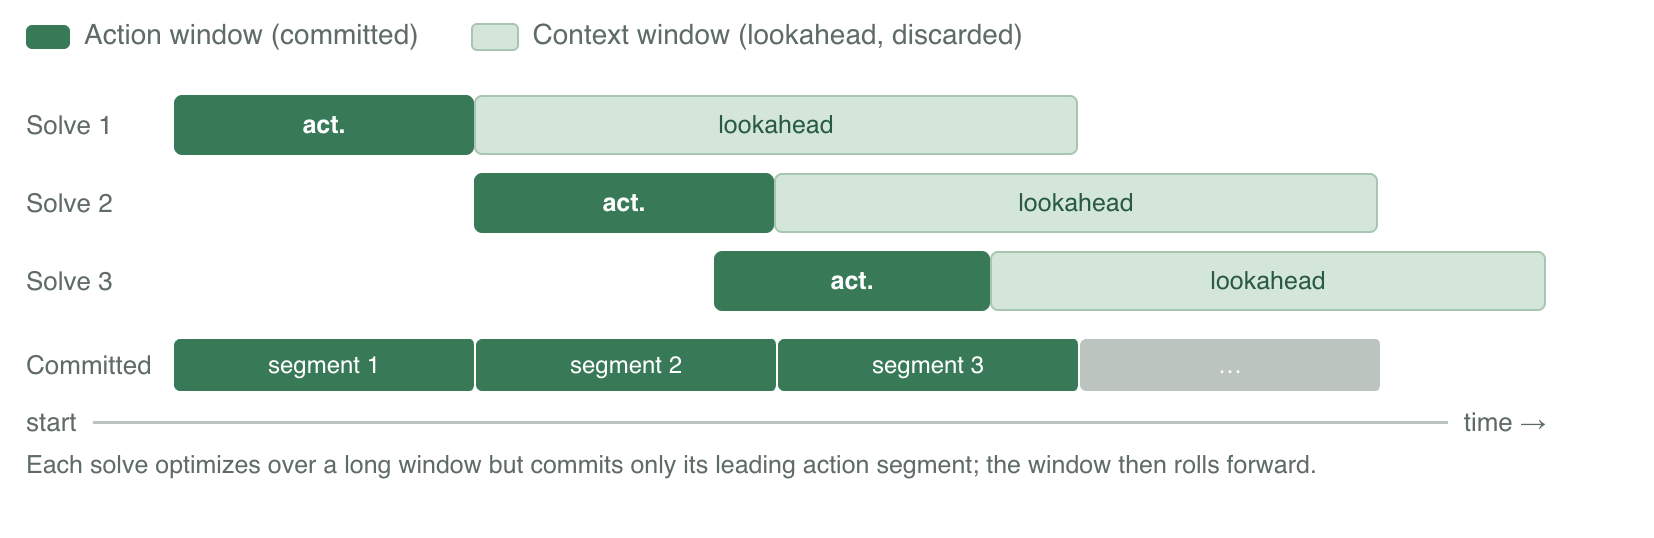
\includegraphics[width=\linewidth]{Figures/rolling_horizon.png}
  \caption{Rolling-horizon decomposition into overlapping windows.}
  \label{fig:rolling-horizon}
\end{figure}

\subsection{Financial indicators for pre-feasibility}

Pre-feasibility analysis translates operating schedules into economic terms. The
core indicators are the \textbf{net present value} (NPV), the \textbf{internal
rate of return} (IRR), and the \textbf{levelized cost} of the output product
(LCOX), all discounted at a \textbf{weighted-average cost of capital} (WACC) and
supported by a full \textbf{discounted-cash-flow} (DCF) statement
(Table~\ref{tab:financial-indicators}). Because
early-stage estimates carry wide accuracy ranges, industry practice formalizes
estimate maturity through cost-estimate classification \cite{aace2020}, and cost
trajectories for renewable generation are tracked by public sources
\cite{irena2023}. These indicators are the raw material that the interpretation
agent must later explain in plain language.

\begin{table}[H]
  \centering
  \small
  \begin{tabularx}{\linewidth}{@{}>{\raggedright\arraybackslash}p{3.9cm} >{\raggedright\arraybackslash}X >{\raggedright\arraybackslash}X@{}}
    \toprule
    \textbf{Indicator} & \textbf{What it measures} & \textbf{Role in pre-feasibility} \\
    \midrule
    Net present value (NPV) & The project's cash flows over its life, discounted to
      today. & Absolute value created; a positive NPV means the project earns above
      its cost of capital. \\
    \addlinespace
    Internal rate of return (IRR) & The discount rate at which the NPV is zero. & A
      single rate to compare against the hurdle rate. \\
    \addlinespace
    Levelized cost of output (LCOX) & Discounted lifetime cost per unit of product
      (hydrogen, ammonia, and so on). & Cost competitiveness of the molecule against
      a benchmark price. \\
    \addlinespace
    Weighted-average cost of capital (WACC) & The blended required return on debt and
      equity. & The rate at which future cash flows are discounted. \\
    \addlinespace
    Discounted cash flow (DCF) & Year-by-year revenue, cost, tax, and net and
      cumulative cash flow, discounted. & The full statement the other indicators
      summarize. \\
    \addlinespace
    Payback period & The time for cumulative discounted cash flow to turn positive. &
      How long invested capital is at risk. \\
    \bottomrule
  \end{tabularx}
  \caption{Financial indicators used in Power-to-X pre-feasibility analysis.}
  \label{tab:financial-indicators}
\end{table}

\subsection{Open frameworks and solvers}

The approach is aligned with a wider movement toward transparent and reproducible
energy-system modeling, exemplified by open frameworks such as \emph{oemof}
\cite{oemof2018} and by calls for openness in the field \cite{pfenninger2018}.
On the solver side, the model can be dispatched through a solver-agnostic
interface such as OR-Tools \cite{ortools} to open-source back ends like the
HiGHS simplex solver \cite{highs2018}, while commercial solvers such as Gurobi
\cite{gurobi2024} remain available for larger instances.

\section{Large language models and agentic systems}
\label{sec:llm-foundations}

\subsection{From language models to reasoning with tools}

Modern large language models (LLMs) are based on the transformer architecture
\cite{vaswani2017} and exhibit strong in-context learning: they adapt to a task
from instructions and examples supplied in the prompt, without retraining.
Prompting techniques such as \textbf{chain-of-thought} improve multi-step
reasoning by eliciting intermediate steps \cite{wei2022cot}. Crucially for this
work, LLMs can be connected to external tools: the \textbf{ReAct} pattern
interleaves reasoning with tool calls so that a model can gather evidence before
answering \cite{yao2023react}, and models can learn to invoke tools with
structured arguments \cite{schick2023toolformer}. This is the mechanism by which
a language model can read facts from a deterministic system rather than inventing
them (Figure~\ref{fig:react-loop}).

\begin{figure}[H]
  \centering
  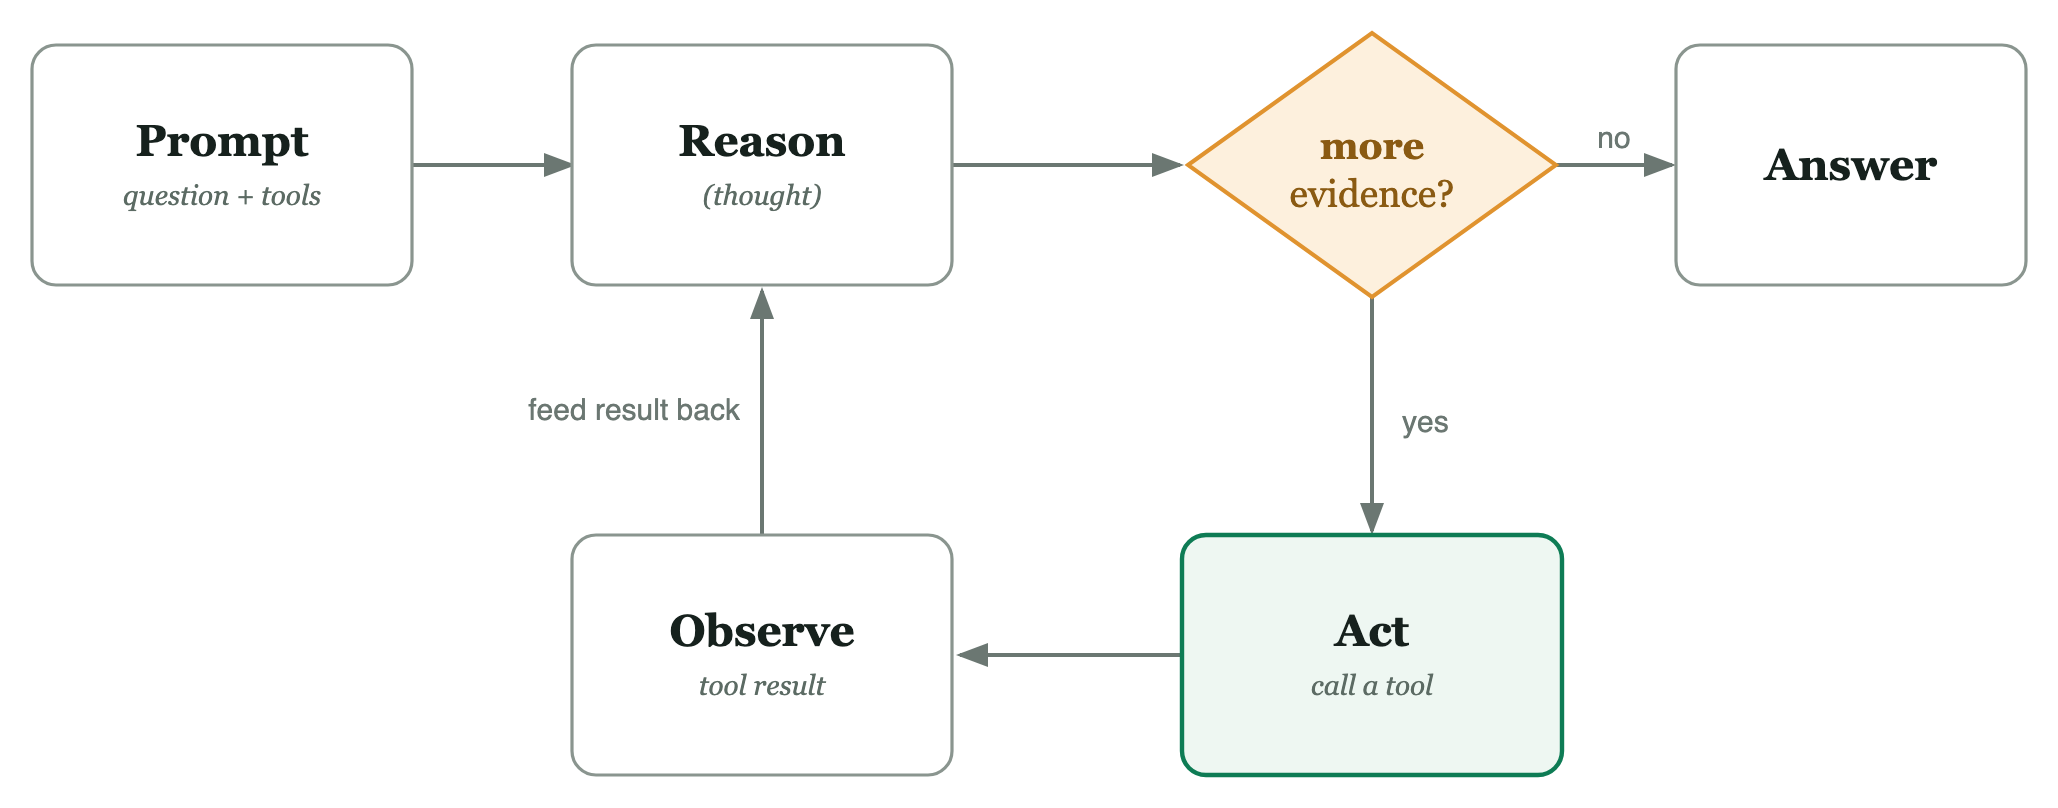
\includegraphics[width=\linewidth]{Figures/react_loop.png}
  \caption{The ReAct pattern: reasoning interleaved with tool calls.}
  \label{fig:react-loop}
\end{figure}

\subsection{Multi-agent orchestration}

Rather than a single monolithic prompt, complex workflows are increasingly built
as \textbf{multi-agent systems}, in which a coordinating agent routes work to
specialized agents, each with a narrow competence and a small tool surface
\cite{wu2024autogen, wang2024survey}. Interoperability between models and tools
is being standardized through protocols such as the \textbf{Model Context
Protocol} (MCP) \cite{mcp2024}, and stateful multi-agent applications can be
expressed as explicit graphs with frameworks such as LangGraph
\cite{langgraph2024}. This director-and-specialists organization
(Figure~\ref{fig:agents}) is the one
adopted by the conversational layer studied in this report.

\begin{figure}[H]
  \centering
  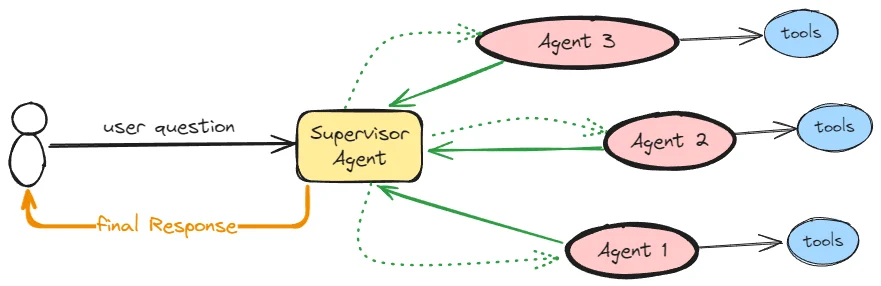
\includegraphics[width=0.9\linewidth]{Figures/agentic_workflow.png}
  \caption{A multi-agent system: a conversation between an orchestrator and specialists.}
  \label{fig:agents}
\end{figure}

\section{Governed agentic assistance for authoritative systems}
\label{sec:governed}

Integrating a probabilistic model into a deterministic analytical product raises
a central tension. A language model is fluent and helpful but may hallucinate,
misread intent, or be manipulated through content hidden in its inputs
\cite{greshake2023}. An analytical product, by contrast, derives its value from
reproducibility and auditability. An autonomous chatbot that silently mutated
assumptions or generated final figures would destroy exactly the property that
makes the tool trustworthy.

The appropriate design is therefore \textbf{bounded orchestration}: the assistant
may reason, retrieve, and propose, but it does not hold authority over state or
over numbers. Four principles enforce this separation. First, a \textbf{read /
write split}: read operations execute immediately, while any state-changing
action becomes a proposal. Second, \textbf{typed proposals}: model output is
converted into a structured, schema-checked payload rather than free text. Third,
\textbf{human-in-the-loop approval}: a user explicitly accepts a proposal before
it mutates the project or launches computation. Fourth, \textbf{deterministic
final authority}: even a successful assisted step only prepares inputs, while the
operational and financial results still come from the optimization engine. To
these, grounding techniques such as retrieval-augmented generation
\cite{lewis2020rag} add the requirement that generated statements be anchored to
retrieved facts rather than to the model's parametric memory. Together, these
principles let assistance improve usability without becoming a source of
numerical truth.

\section{Result interpretation and visualization for analytical software}
\label{sec:interp-foundations}

An analytical tool creates value only when its outputs support a decision. The
study of the existing platform showed that its results were available but not
interpreted: the burden of turning a population of simulations into an
operational and financial story fell entirely on the user. Two complementary
capabilities address this gap.

The first is \textbf{visualization}. Interactive exploration, such as scatter
plots with selectable axes and drill-down financial tables, lets a user compare
scenarios and locate the drivers of value before examining a single run in
detail. Effective visualization is not decoration; it is the interface through
which a large result set becomes legible.

The second is \textbf{grounded natural-language interpretation}. Building on the
tool-augmented reasoning described above, a language model can narrate what a
result means, which configuration produced it, and where its value comes from,
provided every figure it cites is read from the deterministic output rather than
computed by the model. The design challenge is precisely this grounding: the
explanation must be fluent and useful while remaining fully traceable to
simulation facts, with no invented numbers. This combination of interactive
visualization and grounded interpretation is at the heart of the work
detailed in Chapters~4 and~5.

\section{Evaluating and observing LLM-based systems}
\label{sec:eval-foundations}

A capability that relies on a language model cannot be validated by unit tests
alone: the same intent can be phrased in countless ways, and correctness is often
a matter of behavior (grounded, sound, appropriately cautious) rather than an
exact string. Evaluating such systems therefore requires dedicated methods.

For free-text outputs such as interpretations, the \textbf{LLM-as-a-judge}
approach uses an independent model, guided by an explicit rubric, to score
responses along dimensions such as faithfulness to the retrieved data and
soundness of the reasoning \cite{zheng2023judge}. Because a single judgement is
noisy, scores are aggregated over repeated evaluations and tracked across
versions. For structured outputs such as a generated topology, comparison against
a reference is better captured by a structural metric: the \textbf{graph edit
distance} measures the minimum number of edits needed to turn one graph into
another \cite{sanfeliu1983}, giving a fidelity score that plain string matching
cannot. These offline methods are complemented by \textbf{observability}: tracing
every model call, tool invocation, cost, and evaluator score, so that behavior
can be inspected, debugged, and compared in production, for which open platforms
such as Langfuse are designed \cite{langfuse2025}. Together these methods form
the methodology behind the evaluation harness developed in this work
(Figure~\ref{fig:eval-methods}).

\begin{figure}[H]
  \centering
  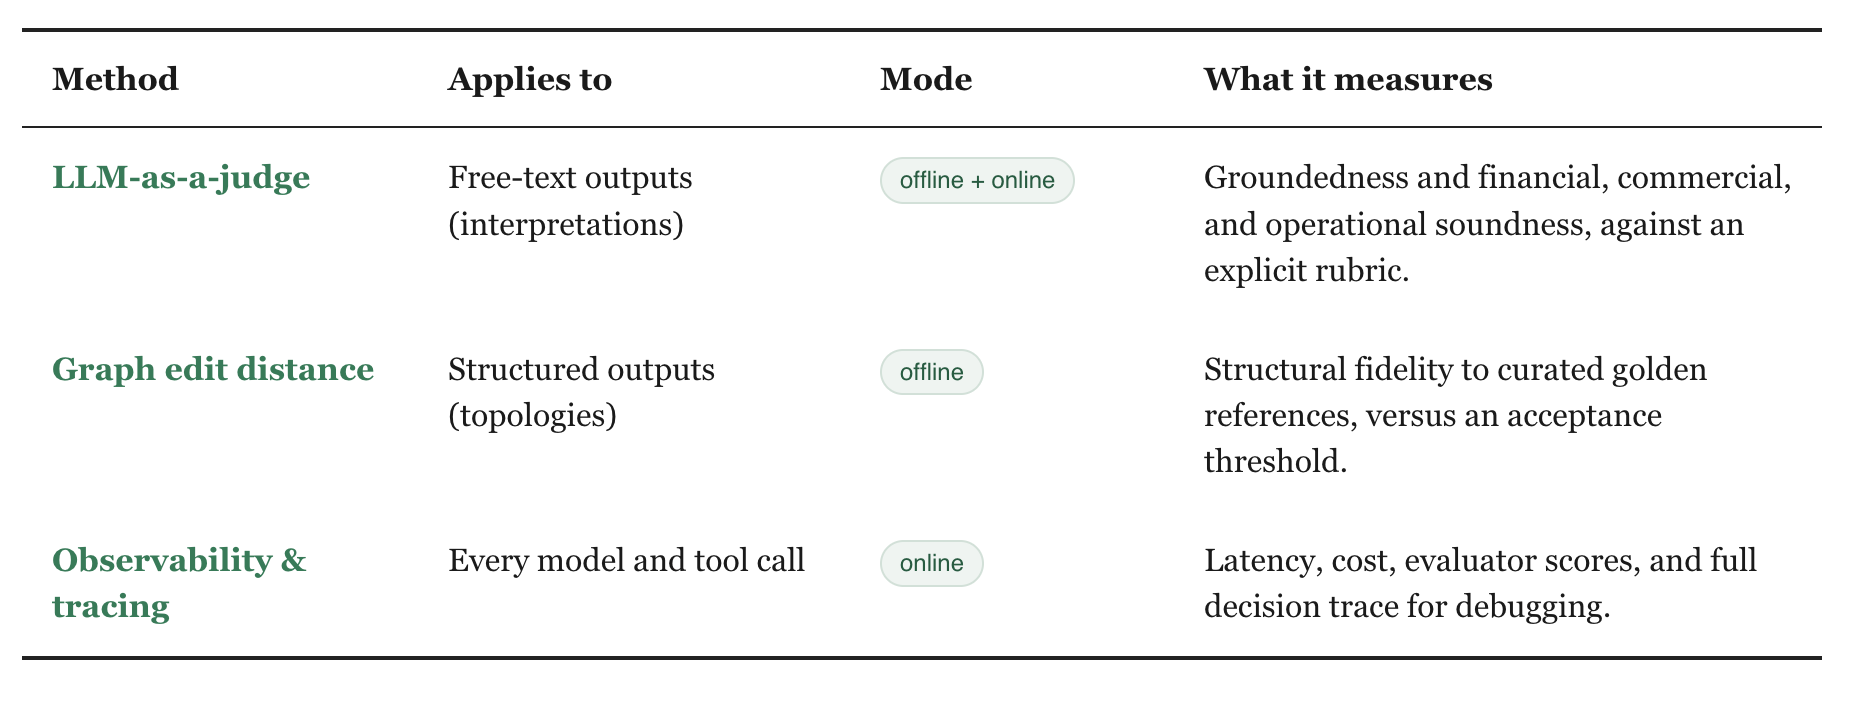
\includegraphics[width=\linewidth]{Figures/evaluation_methods.png}
  \caption{Complementary methods for evaluating the assisted capabilities.}
  \label{fig:eval-methods}
\end{figure}

\section{Enterprise foundations}
\label{sec:enterprise-foundations}

Two further axes frame the platform work carried out by the team. On identity,
enterprise analytical tools are expected to delegate authentication to a
federated identity provider through standard protocols such as OpenID Connect,
rather than operating a self-hosted identity stack, which reduces the security
surface owned by the application. On delivery, modern products rely on
infrastructure-as-code, automated builds and tests, container images, and
operational monitoring to remain deployable and reproducible. For an internal
product adapted across several clients, these are product requirements rather
than one-off engagement concerns: they determine whether the same core can be
delivered reliably to each new adaptation.

\section{Benchmarking and technical justification}
\label{sec:benchmark}

The direction can be justified by comparing candidate approaches against the
requirements observed in the existing platform. No isolated approach satisfies
the analytical, usability, trust, and operational requirements at the same time.
Table~\ref{tab:benchmark} summarizes the comparison.

\begin{table}[H]
  \centering
  \small
  \begin{tabularx}{\linewidth}{@{}>{\raggedright\arraybackslash}p{3.2cm} >{\raggedright\arraybackslash}X >{\raggedright\arraybackslash}X@{}}
    \toprule
    \textbf{Approach} & \textbf{Main limitation} & \textbf{Implication for the ETO} \\
    \midrule
    Manual / spreadsheet analysis & Flexible but weak in traceability, scalability,
      and reproducibility. & Useful for early reasoning, unsuitable as the
      computational authority. \\
    \addlinespace
    Solver-backed optimization & Strong numerical authority but insufficient alone
      for guidance, security, and usability. & Preserve the deterministic engine;
      improve the surrounding product. \\
    \addlinespace
    Cloud-native platform practices & Improve delivery reliability but do not solve
      modeling or interpretation. & Use as an engineering foundation for
      maintainable evolution. \\
    \addlinespace
    Self-hosted identity & Provides control but increases the security surface and
      operational burden. & Replace with federated enterprise OIDC. \\
    \addlinespace
    Workflow-oriented UX & Improves adoption but must stay connected to model
      constraints and validation. & Redesign the interface around guided workflows. \\
    \addlinespace
    Autonomous LLM chatbot & Improves interaction but can hallucinate or silently
      mutate state. & Reject autonomy; adopt bounded, approval-gated assistance. \\
    \addlinespace
    \textbf{Governed agentic assistance} & Requires careful design of tools,
      validation, and evaluation. & \textbf{The chosen direction}: assist without
      holding numerical authority. \\
    \bottomrule
  \end{tabularx}
  \caption{Comparison of candidate approaches.}
  \label{tab:benchmark}
\end{table}

The comparison shows that the appropriate response is not a single technology but
a combination that matches each requirement to the right solution family. That
combination is the target direction set out next.

\section{Target direction: governed modernization}
\label{sec:target}

The chosen direction is a \textbf{governed modernization} of the existing
platform rather than a rewrite: it preserves what is sound and redesigns what
limits adoption, across five decisions.

\begin{itemize}
  \item \textbf{Preserve the deterministic core} as the sole source of numerical
    truth; assisted work prepares inputs and explanations, never final results.
  \item \textbf{Restore the engineering and deployment foundation}, with
    reproducible delivery, infrastructure-as-code, and operational observability.
  \item \textbf{Migrate to federated enterprise identity} (OIDC), removing the
    self-hosted identity surface from the application stack.
  \item \textbf{Redesign the experience around guided workflows}, making the
    model easier to use without hiding its constraints or its validation.
  \item \textbf{Introduce governed agentic assistance}: typed proposals, system
    validation, and explicit human approval before any state change, with the
    optimizer retaining numerical authority.
\end{itemize}

\section{Positioning of the work}
\label{sec:positioning}

Within this direction, the work presented in this report concentrates on
the axes where the existing platform was weakest and where language models offer
the most leverage. The gap is not the solver but the product around it, and in
particular two of its facets: results that were produced but not interpreted, and
an assistant capability that, to be trustworthy, must be measured rather than
assumed.

Accordingly, the three pillars developed in the following chapters are the
\textbf{result-interpretation agent} (a grounded, read-only explainer of
simulation economics), the \textbf{visualization layer} that surfaces and
supports that interpretation, and the \textbf{evaluation harness} that measures
the grounding and soundness of the explanations produced. Each rests directly on
the foundations laid in this chapter: techno-economic indicators to be explained,
tool-augmented and governed language-model reasoning, and dedicated evaluation and
observability methods.

\section*{Conclusion}

This chapter studied the existing Energy Transition Optimizer, established the
technical foundations of the project axis by axis, and justified the choice of a
governed modernization that preserves the deterministic core while making it
accessible and trustworthy. It also positioned the work around result
interpretation, visualization, and evaluation. The next chapter turns this
positioning into an explicit specification of the functional and non-functional
requirements.
